\makeatletter
\makeatother
\documentclass[10pt,english]{article}\usepackage{graphicx, color}
%% maxwidth is the original width if it is less than linewidth
%% otherwise use linewidth (to make sure the graphics do not exceed the margin)
\usepackage{alltt}
\usepackage[T1]{fontenc}
\usepackage[latin9]{inputenc}
\usepackage{geometry}
\geometry{left=1.5cm,right=1.5cm,top=2cm,bottom=2cm}
\usepackage{fancyhdr}
\pagestyle{fancy}
\setlength{\parskip}{\smallskipamount}
\setlength{\parindent}{0pt}
\usepackage{amsthm}
\usepackage{amsmath}
\usepackage{subfigure}

\makeatletter

%%%%%%%%%%%%%%%%%%%%%%%%%%%%%% LyX specific LaTeX commands.
\providecommand{\LyX}{L\kern-.1667em\lower.25em\hbox{Y}\kern-.125emX\@}

%%%%%%%%%%%%%%%%%%%%%%%%%%%%%% Textclass specific LaTeX commands.
\numberwithin{equation}{section}
\numberwithin{figure}{section}

\@ifundefined{date}{}{\date{}}
%%%%%%%%%%%%%%%%%%%%%%%%%%%%%% User specified LaTeX commands.
\pagestyle{empty} 

\makeatother

\usepackage{babel}
\begin{document}

\title{Week8 Report}


\author{Xiaohui Li, Luhuan Wu}

\maketitle


In this week, we further study the ranking node effect on short average path. We focus on the extreme cases. In the first step, we check the feasibility of the new degree sequence model. Then we study the effect on average short path in graph. 

\section{Average short path}
For this part, we study the marginal node effect upon average short path based upon page rank, betweenness centrality, total degree, in degree and out degree ranking. We test for the small graph (expected mean equals to 3), and medium graph (10).\\
\subsection{Small graph}
We first test the graph where in-degree and out-degree are correlated, perfectly correlated and independent. \\
\subsubsection{General case}
\begin{figure}[htbp]
\centering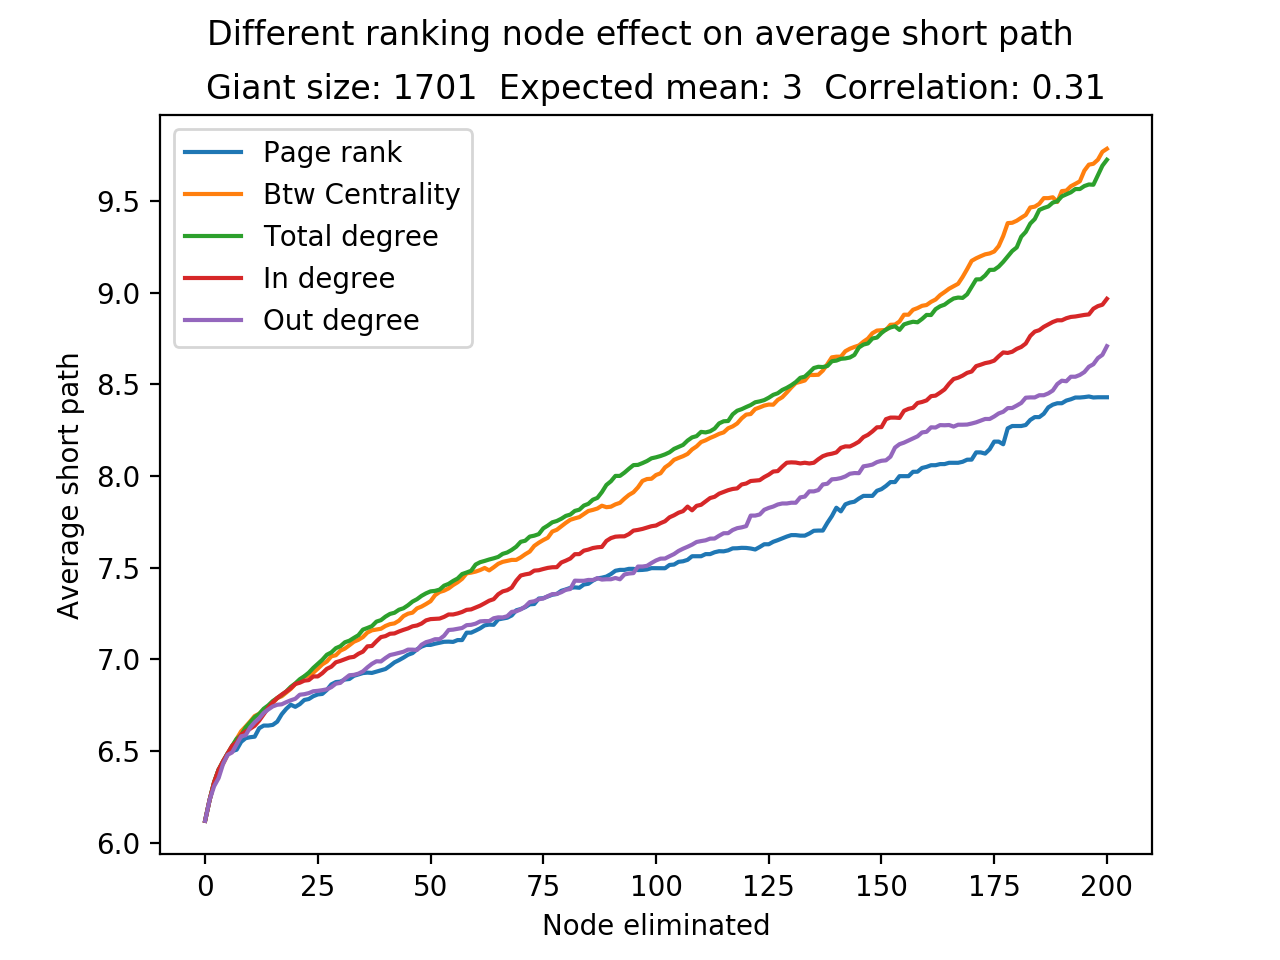
\includegraphics[width=10cm, height=8cm]{3_corr}
\caption{Node effect on average shortest path}
\end{figure}
\quad\\
\quad\\


\subsubsection{Perfectly correlated}
\quad\\

\begin{figure}[htbp]
\centering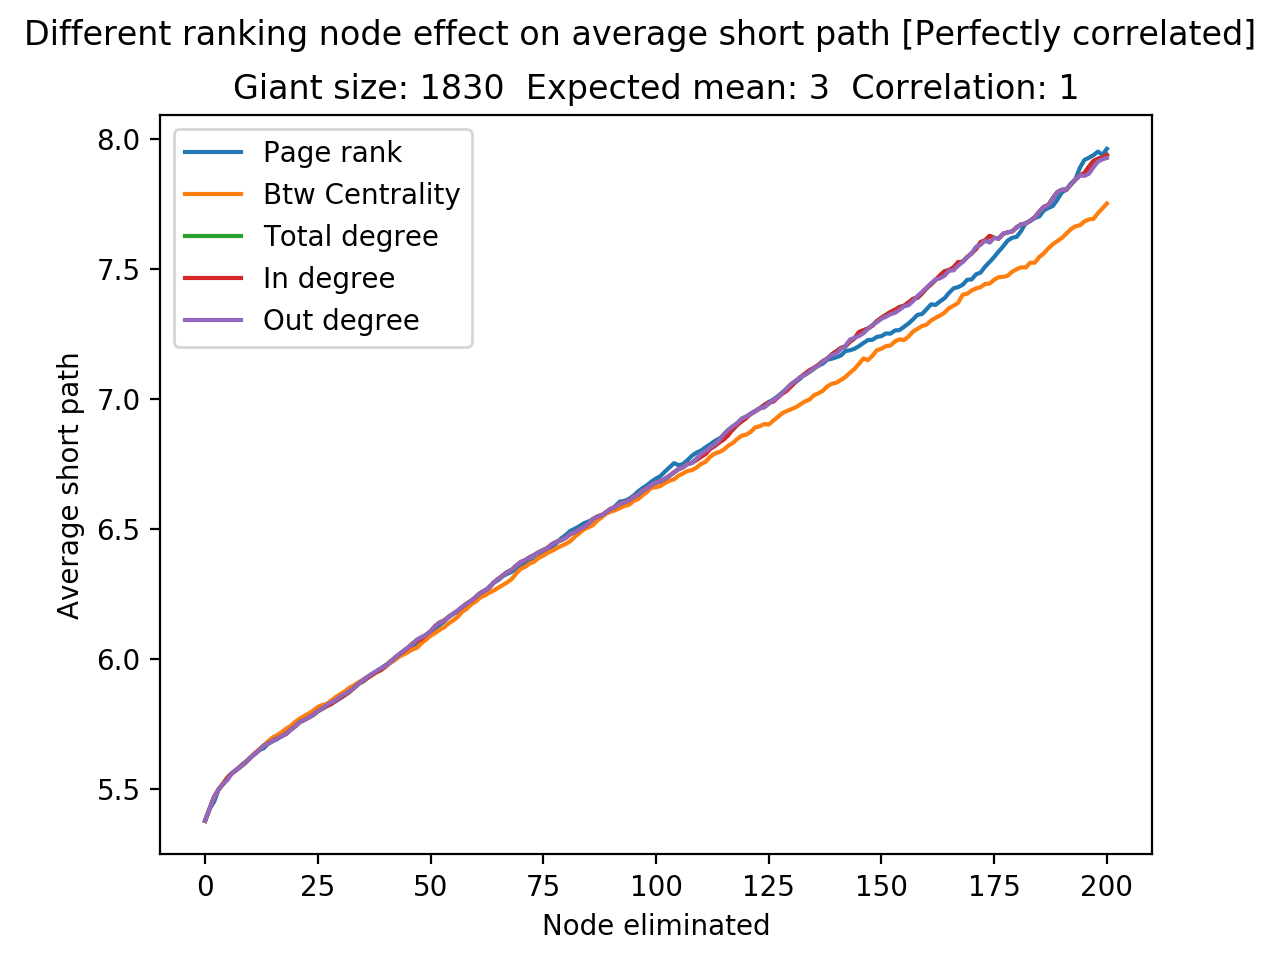
\includegraphics[width=10cm, height=8cm]{3_sam}
\caption{Perfectly correlated node effect on average shortest path}
\end{figure}
\quad\\


\subsubsection{Independent}
\begin{figure}[htbp]
\centering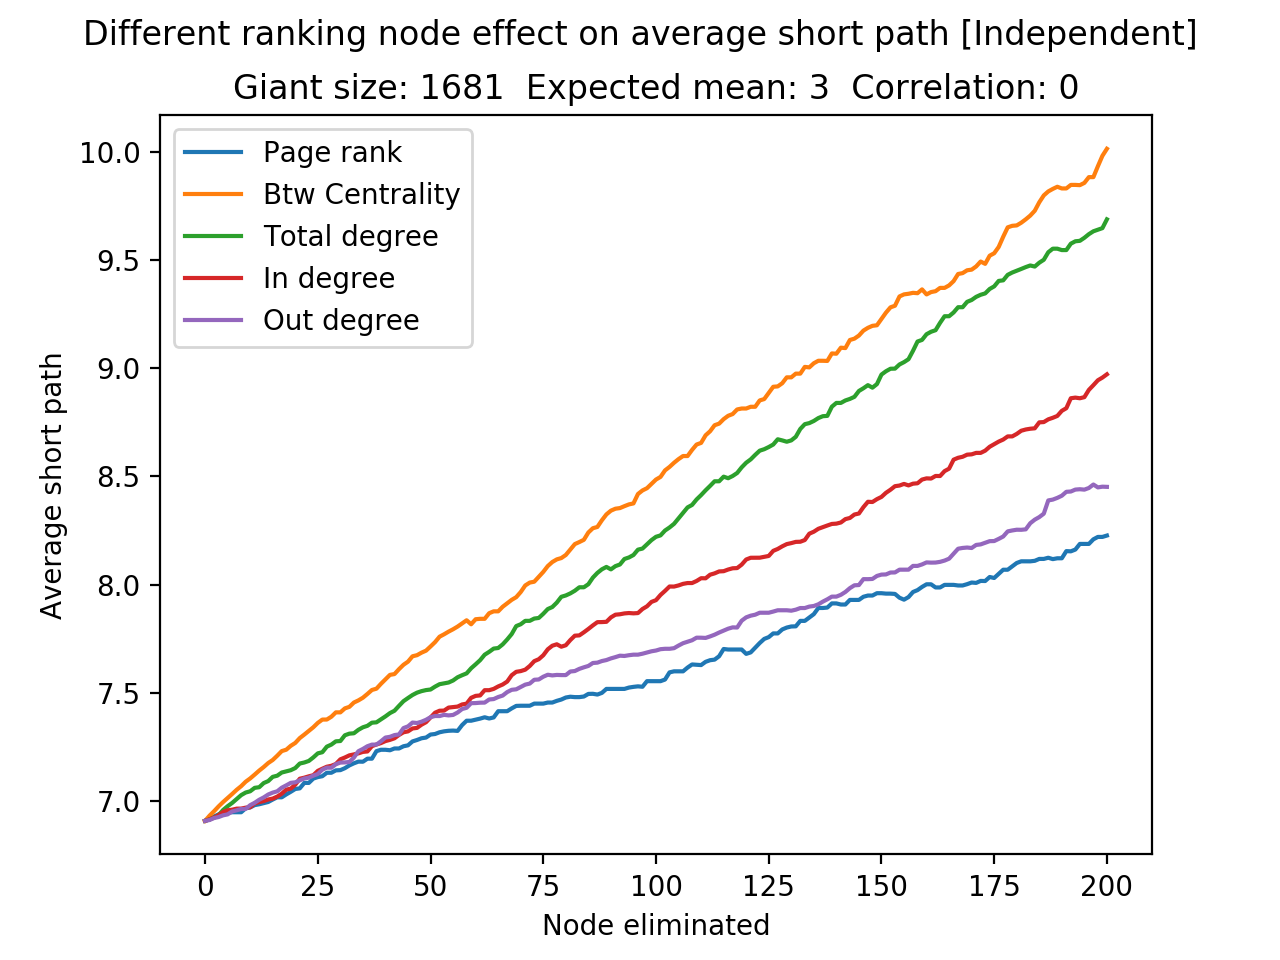
\includegraphics[width=10cm, height=8cm]{3_ind}
\caption{Independent degree sequence node effect on average shortest path}
\end{figure}
\quad\\


\subsection{Mediuml graph}
We test the graph where expected degree is 10. 
\subsubsection{General case}
\begin{figure}[htbp]
\centering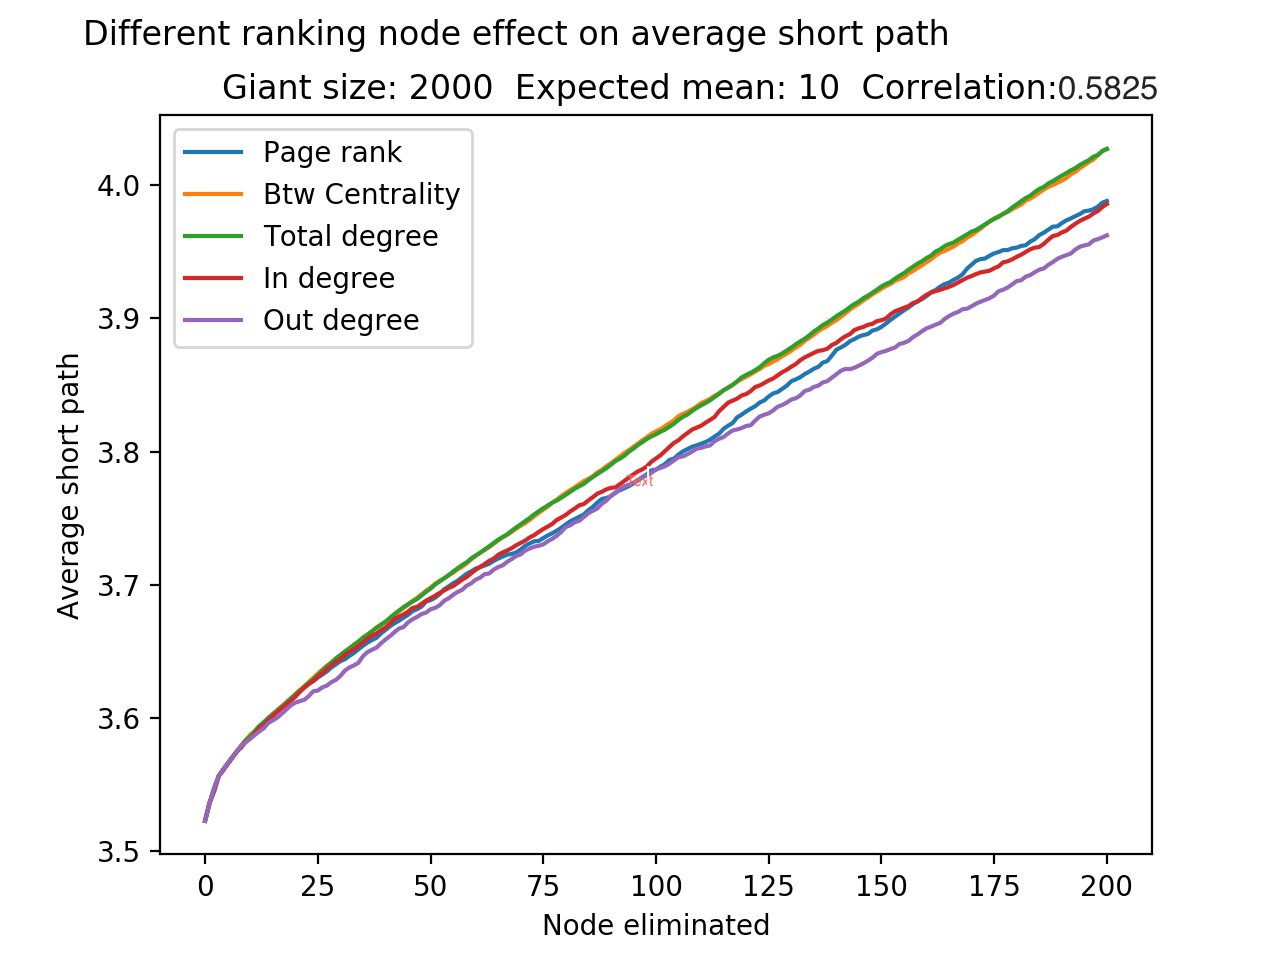
\includegraphics[width=10cm, height=8cm]{10_corr}
\caption{Node effect on average shortest path}
\end{figure}
\quad\\


\subsubsection{Perfectly correlated}

\begin{figure}[htbp]
\centering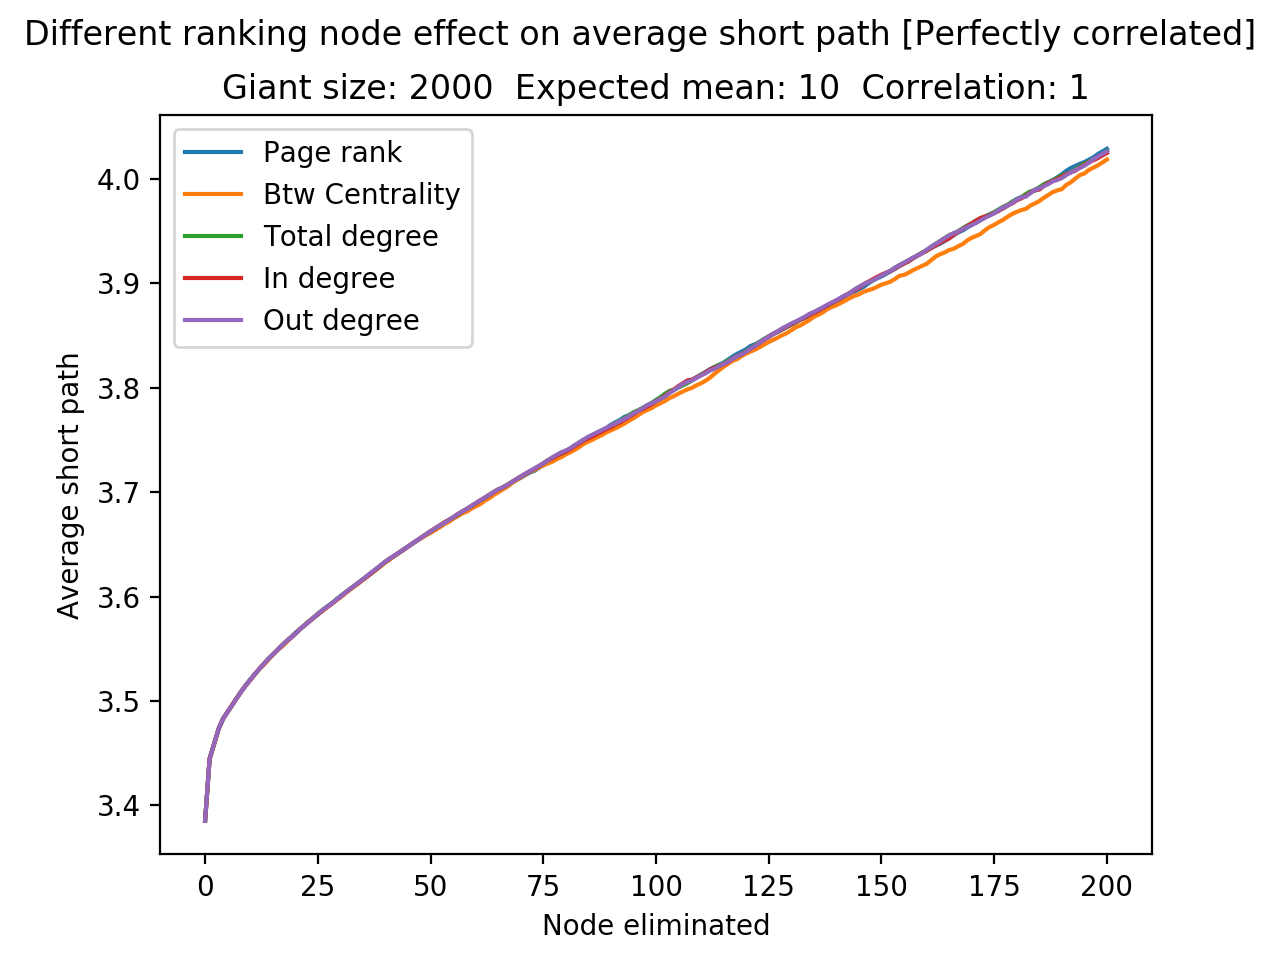
\includegraphics[width=10cm, height=8cm]{10_sam}
\caption{Perfectly correlated node effect on average shortest path}
\end{figure}
\quad\\


\subsubsection{Independent}
\begin{figure}[htbp]
\centering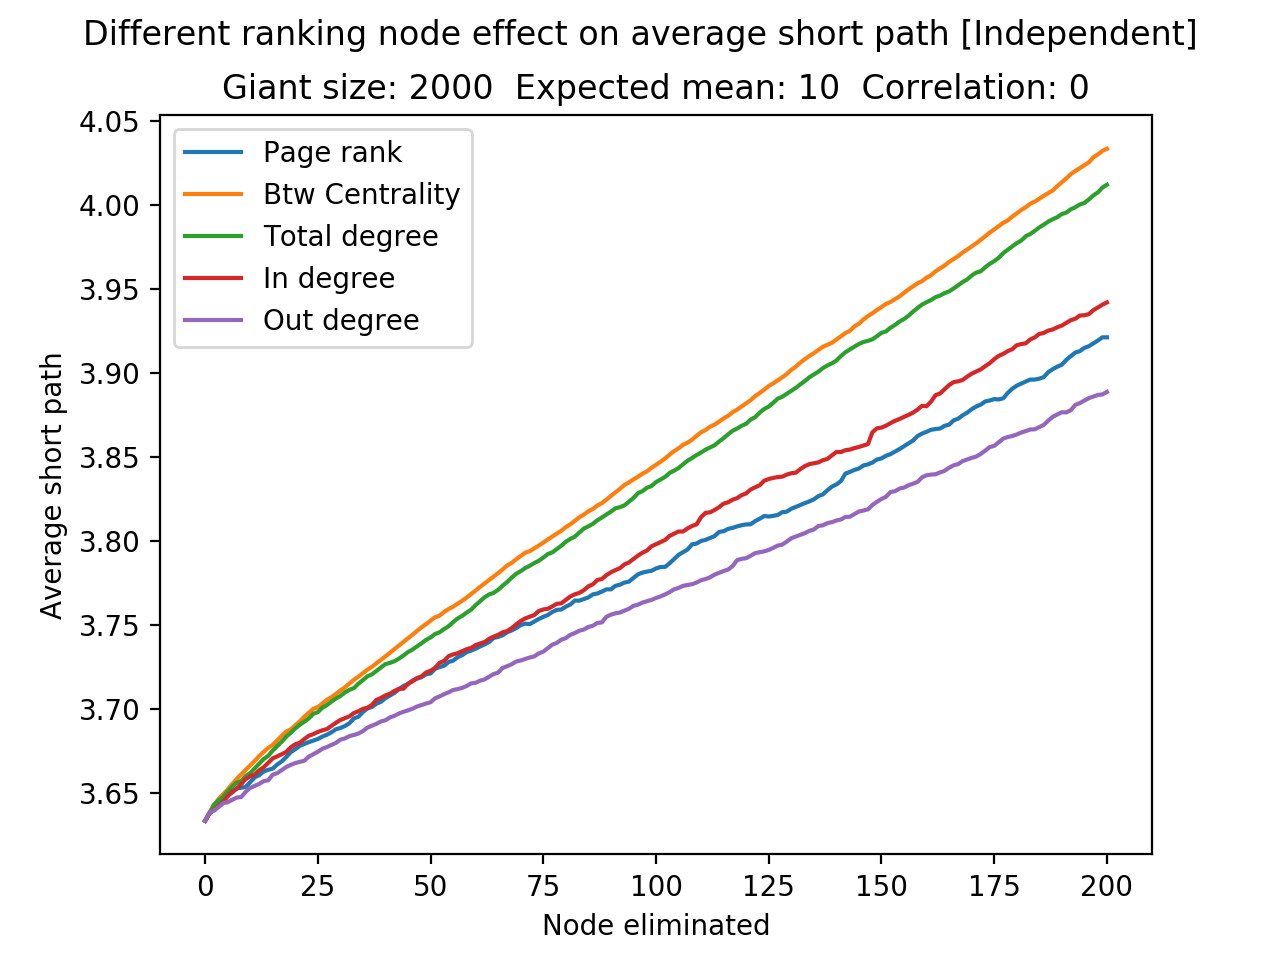
\includegraphics[width=10cm, height=8cm]{10_ind}
\caption{Independent degree sequence node effect on average shortest path}
\end{figure}
\subsection{Large graph}
We test the graph where expected degree is 20. 
\subsubsection{General case}
\begin{figure}[htbp]
\centering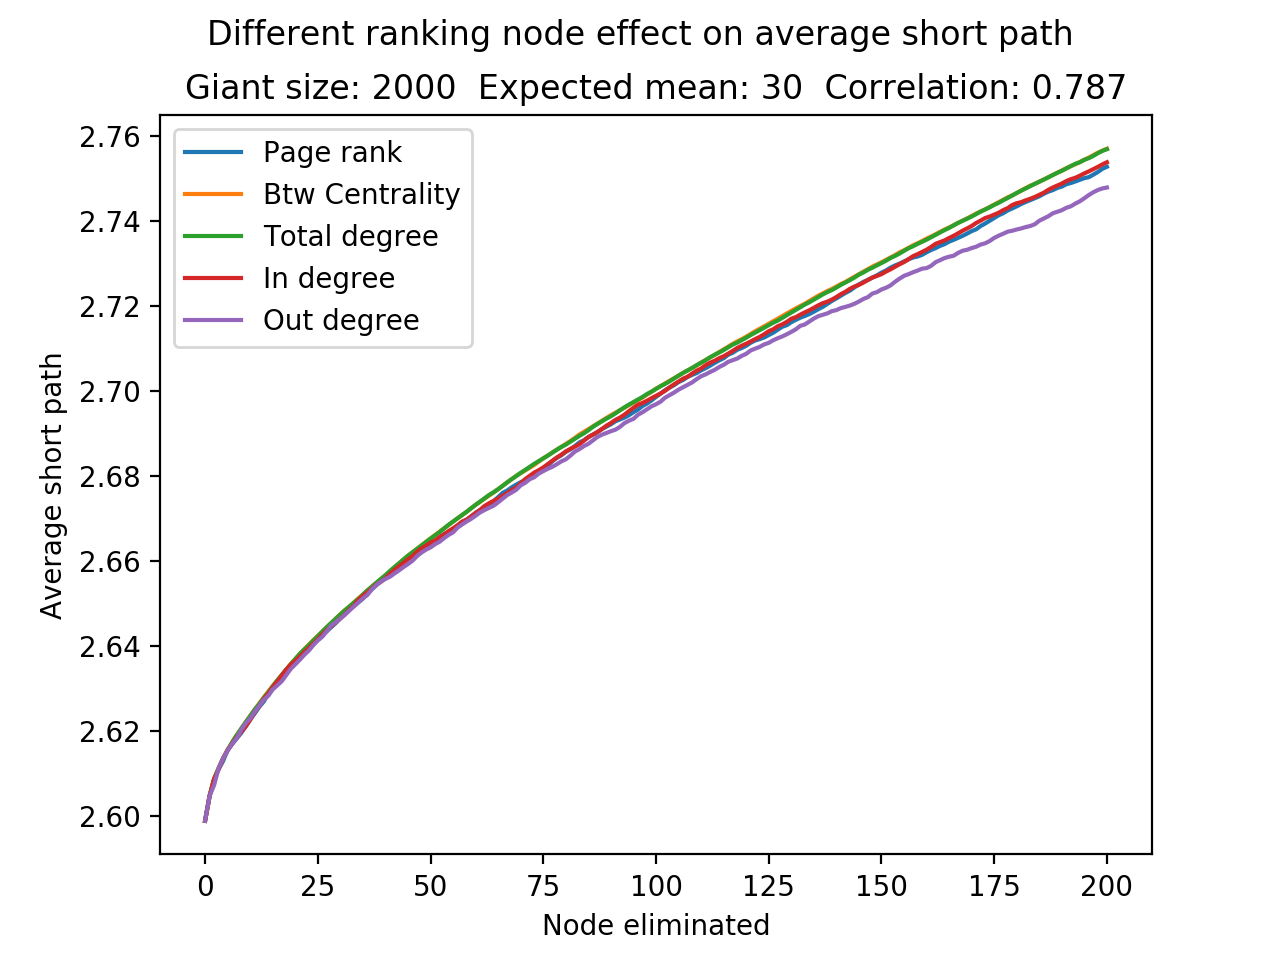
\includegraphics[width=9cm, height=7cm]{30_cor}
\caption{Node effect on average shortest path}
\end{figure}
\quad\\


\subsubsection{Perfectly correlated}

\begin{figure}[htbp]
\centering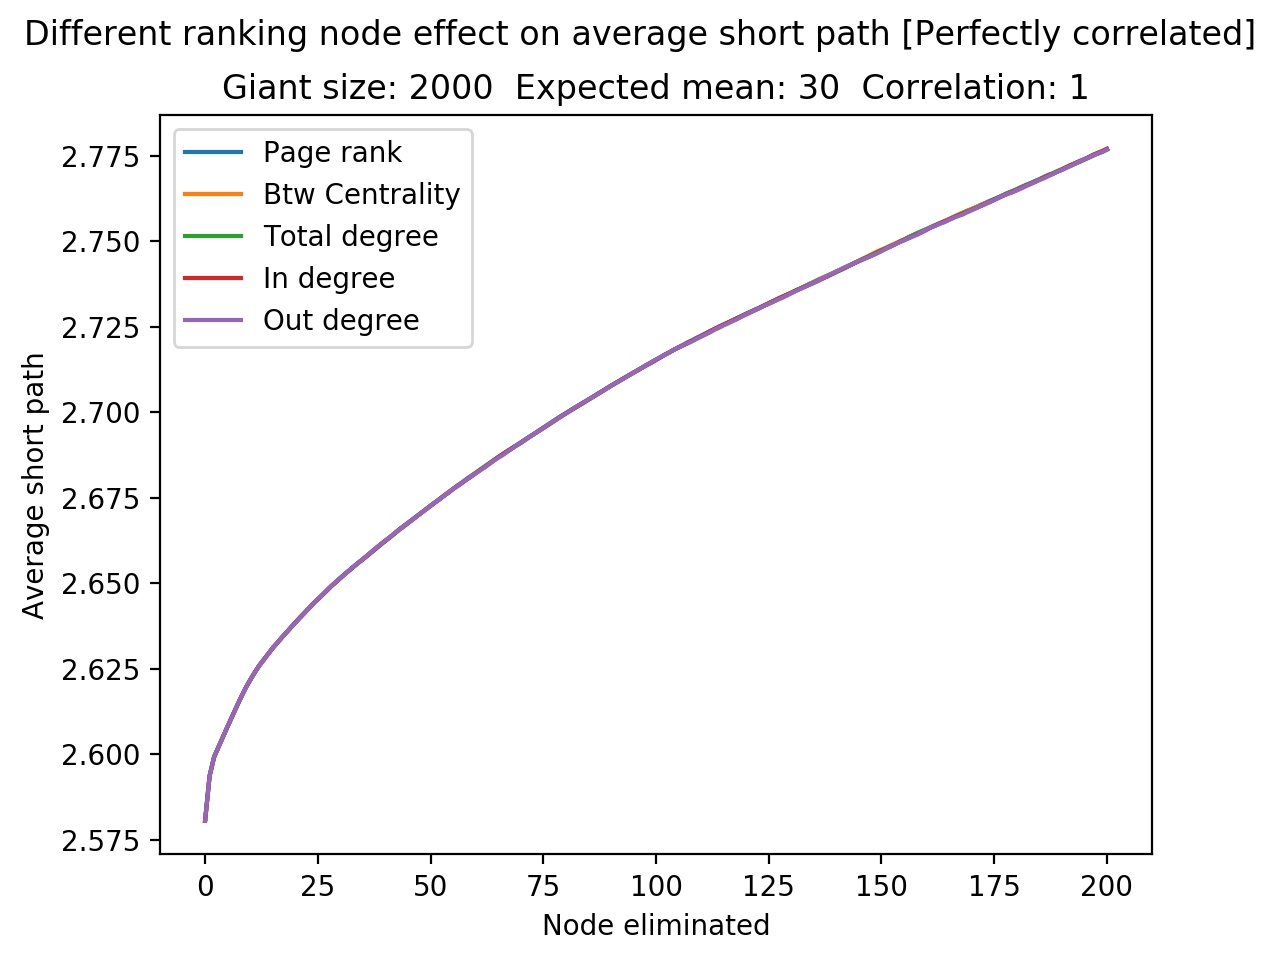
\includegraphics[width=10cm, height=8cm]{30_sam}
\caption{Perfectly correlated node effect on average shortest path}
\end{figure}
\quad\\


\subsubsection{Independent}
\begin{figure}[htbp]
\centering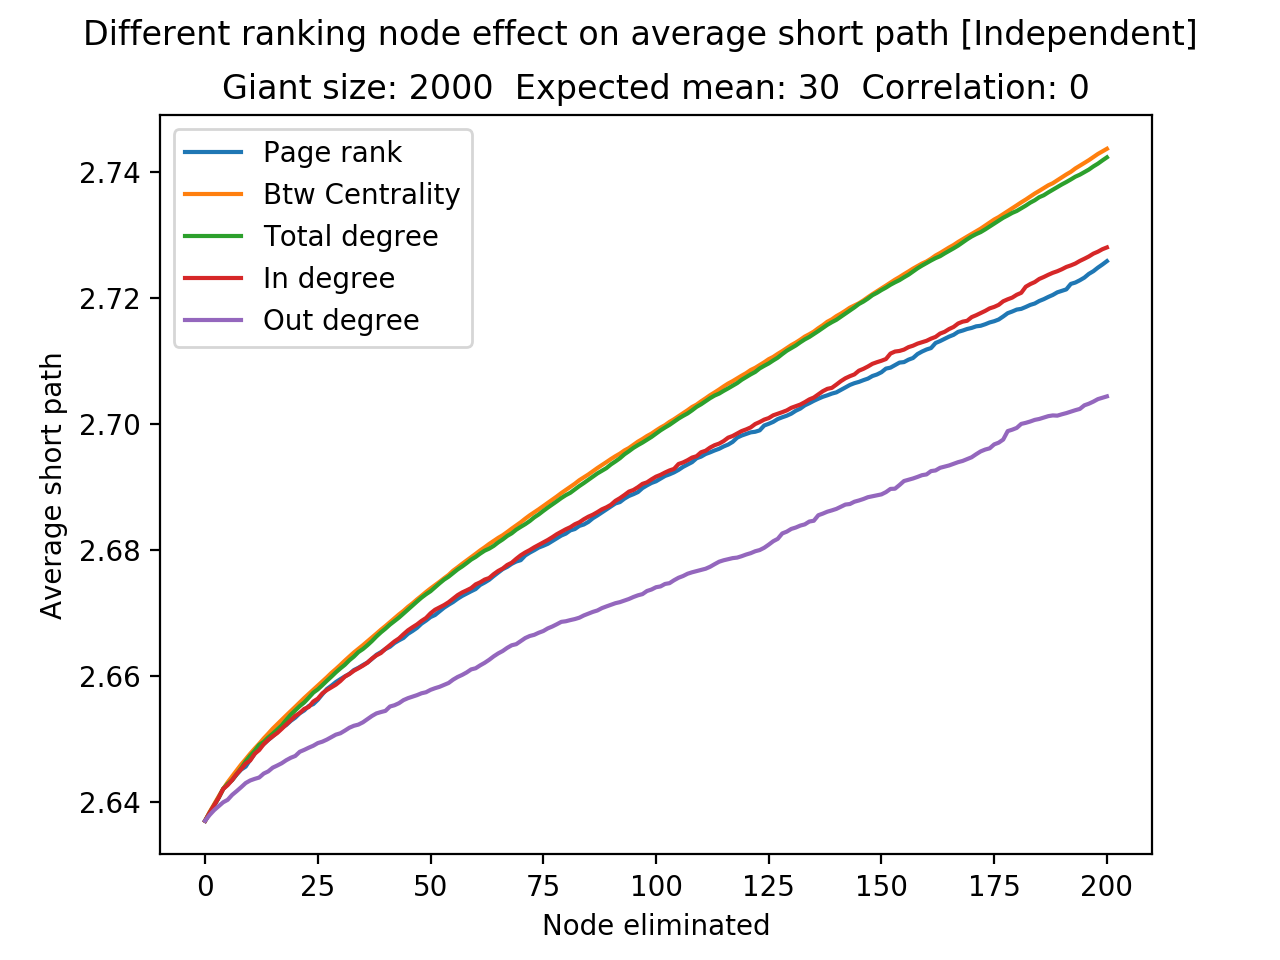
\includegraphics[width=10cm, height=8cm]{30_ind}
\caption{Independent degree sequence node effect on average shortest path}
\end{figure}
\quad\\



\subsubsection{Conclusion}
From the empirical result, the performance of page rank and betweenness centrality ranking on average short path depends on the correlation between in-degree and out-degree sequence. With highly correlated degree, the generated directed configuration graph's page rank and betweenness centrality's effect on average short path are much similar, whereas in independent case, the page rank is less effective as betweenness. The total degree always keep highly similar effect with betweenness centrality.

\end{document}



